\documentclass[12pt,letter]{article}
\usepackage[moduleName={Super VCA}]{KautenjaDSP}
\begin{document}
\titlePage{img/Logo}{img/Module}{img/KautenjaDSP}

% -------------------
% MARK: Overview
% -------------------

\section{Overview}

Super VCA is an emulation the Gaussian Interpolation filter effect from the S-SMP sound chip on the Super Nintendo Entertainment System (SNES). The Gaussian Interpolation filter of the S-SMP chip was applied to BRR samples to remove unpleasant high-frequency content from the audio signal. Super VCA provides the key features of the Gaussian filter of the S-SMP chip,
namely,
\begin{itemize}
  \item \textbf{Stereo Processing:} Two lanes of processing for stereo effects or other creative applications
  \item \textbf{Input Gain:} Amplify input signals up to $6dB$ and attenuate signals to $-\infty dB$ with the gain control
  \item \textbf{Four Filter Modes:} Four filter modes that act as different combinations of the two coefficients for the reconstruction filter.
  \item \textbf{Filter Rate Control:} Knob and CV control of the Gaussian interpolation filter's rate, which introduces weird distortion and aliasing effects.
  \item \textbf{Bypass:} Bypass control to pass the gained signal through the VCA
\end{itemize}

\begin{figure}[!b]
\centering
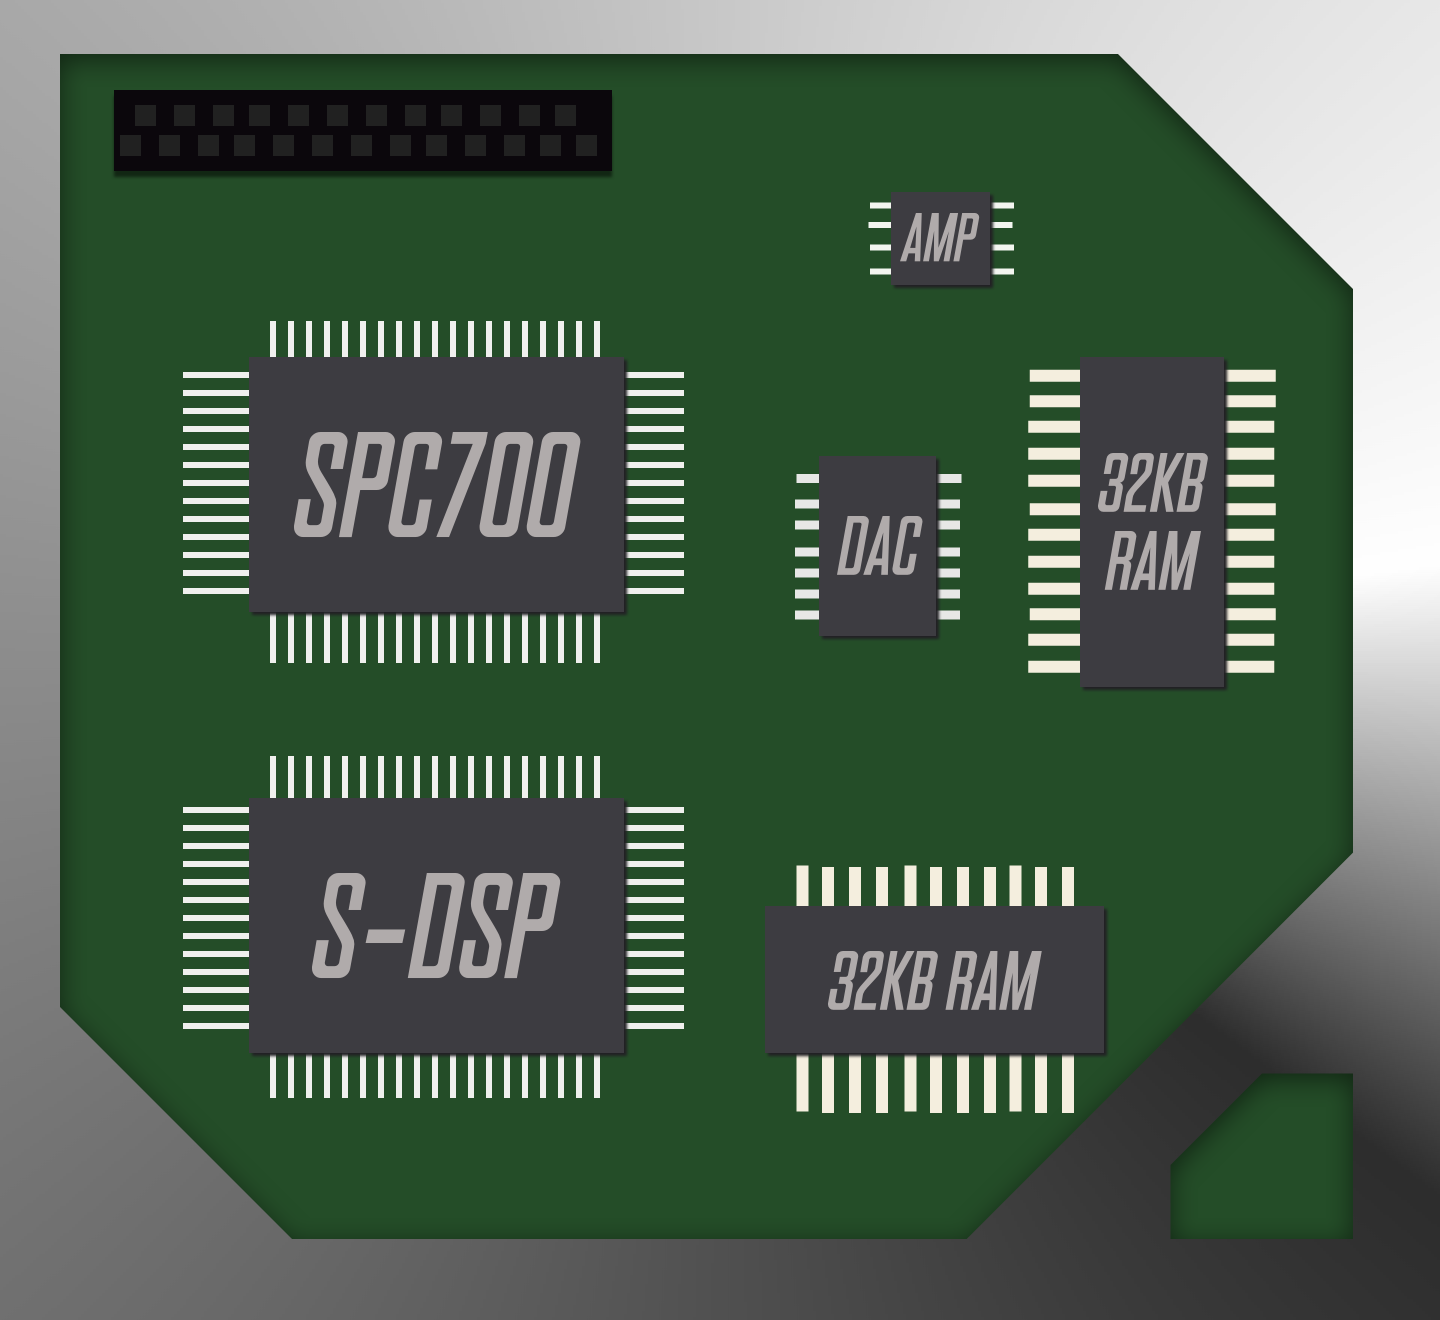
\includegraphics[width=0.5\textwidth]{img/Chip}
\caption*{\small The S-SMP module from the SNES. The S-SMP included two discrete microprocessors: the SPC700, and the S-DSP. The SPC700 performed primary computation, while the S-DSP performed DSP specific computations, like BRR decoding, sample playback, applying the echo effect, mixing levels, etc. The SPC700 and S-DSP shared $64KB$ of total RAM that was used for BRR sample data and the echo buffer. The digital audio is decoded back to an analog signal by a 16-bit DAC and amplified using an Op-Amp. Before digital-to-analog conversion, the output audio is low-pass filtered by a Gaussian filter that gives the S-SMP chip a distinctive sound.}
\end{figure}

% -------------------
% MARK: Panel Layout
% -------------------

\clearpage
\section{Panel Layout}

\begin{figure}[!htp]
\centering
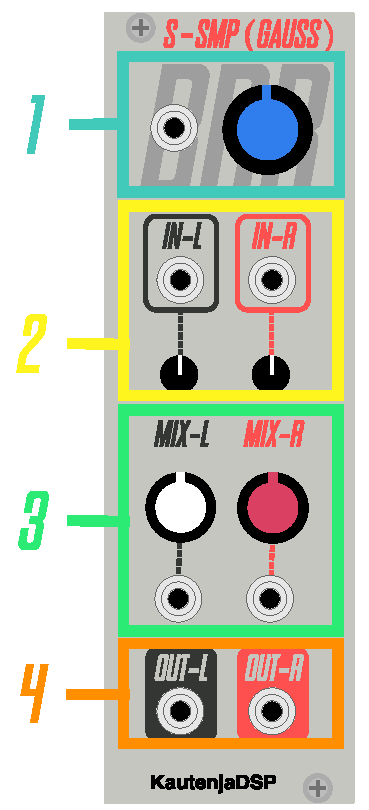
\includegraphics{img/Interface}
\end{figure}

\subsection{Audio Input}

The module accepts both mono and stereo inputs. If an input is patched to the left input, but not the right input, the signal is normalled from the left input to the right input. The trimpot acts as a gain control for the individual processing lanes in the range of $[-\infty, 6]dB$. VU meter lights measure the input of individual processing lanes going from off ($-\infty dB$ to $-12dB$), to green ($-12dB$ to $0dB$), and lastly to red ($0dB$ to $6dB$) when clipping begins to occur. Input voltages are clipped to $10V_{pp}$ (i.e., $[-5, 5]V$) for digital processing in the S-SMP emulation. When using Super VCA for audio rate signals in the standard $10V_{pp}$ range, $0dB$ gain will fully saturate the signal\footnote{Some oscillators produce band-limited signals that are mostly $10V_{pp}$, but may have some time-domain ripples outside this range that will be clipped. This will introduce aliasing.}. If using the module to attenuate control voltages in the range of $[-10, 10]V$, a gain setting of at most $-6dB$ is optimal to prevent clipping the signal.

\subsection{Amplifier}

When no input is connected, the trimpot controls the volume level with 8-bit signed resolution (i.e., $\in [-128, 127]$). Negative volumes will invert the phase of the waveform, and can be used for interesting surround sound effects when modulated independently between the stereo pair. When an input is patched to the port, the trimpot acts like an attenuverter that polarizes and scales the CV control over the volume level.

\subsection{Gaussian Interpolation Filter}

The Gaussian Interpolation filter removes high-frequency content and accounts for artifacts of the BRR compression scheme used in the S-SMP chip. There are four ``modes'' of the filter that change the IIR coefficients to produce different effects. The modes are normally meant to be programmed to match audio samples one-by-one, but sound interesting when used for extended phrases. The most noticeable difference between the four modes when using them for extended phrases is the amount of attenuation applied to the input signal. To account for the exponential levels of attenuation that occur, Super VCA introduces an loudness compensation mechanism to boost quieter filter modes. The active filter mode is described by the LED, and can be cycled using the button. Table~\ref{tab:filter-modes} describes the association between the filter modes and the LED colors.

\begin{table}[!htp]
\centering
\caption{The modes of the Gaussian interpolation filter.}
\label{tab:filter-modes}
\begin{tabular}{|c|l|}
\hline
 \bfseries Color                                           & \bfseries Mode \\
\hline\hline
 \tikz\draw[black,fill=red!70!white] (0,0) circle (1ex);          & Loud           \\
\hline
 \tikz\draw[black,fill=green!60!white] (0,0) circle (1ex);  & Weird          \\
\hline
 \tikz\draw[black,fill=blue!70!white] (0,0) circle (1ex); & Quiet          \\
\hline
 \tikz\draw[black,fill=black] (0,0) circle (1ex);  & Barely Audible \\
\hline
\end{tabular}
\end{table}

The Gaussian interpolation filter is normally clocked by the rate of the BRR sample player of the S-SMP chip. Super VCA exposes the control of this filter rate with trimpots that independently control the coarse frequency of the filter rate for each processing lane\footnote{The frequency control does not act as a cut-off frequency, but instead controls the fundamental frequency of the Gaussian interpolation filter.}. Frequency is quantized to a 16-bit value. The ports provide an exponential $V$/Octave input for controlling the pitch of the filters. Inputs are normalled forward from the left lane to the right lane.

\subsection{Audio Output}

Each processing lane produces an output signal of at most $10V_{pp}$ (i.e., $[-5, 5]V$) when the internal amplifier is maxed out. However, due to the loudness compensation mechanism, additional saturation can happen up to $16V_{pp}$ (i.e., $[-8, 8]V$), after which hard clipping will occur. This is mostly noticeable when using the filter in the ``\textit{Weird}'' mode, which has a pretty weird frequency response. VU meter lights measure the output of individual channels going from off ($-\infty dB$ to $-12dB$), to green ($-12dB$ to $0dB$), and lastly to red ($0dB$ to $6dB$) when clipping begins to occur.

\subsection{Bypass}

The bypass switch allows the circumvention of the S-SMP Gaussian interpolation filter emulation without breaking the stereo signal path. When the bypass switch is pointing up, the input signals only pass through the gain circuit before passing to their respective outputs. When the bypass switch is pointing down, the gained inputs pass through the S-SMP Gaussian interpolation filter emulation.

\end{document}
